\documentclass[a4paper,12pt,titlepage,finall]{article}

\usepackage[T1,T2A]{fontenc}     % форматы шрифтов
\usepackage[utf8]{inputenc}      % кодировка символов, используемая в данном файле
\usepackage[english, russian]{babel}      % пакет русификации
\usepackage{tikz}                % для создания иллюстраций
\usepackage{pgfplots}            % для вывода графиков функций
\usepackage{geometry}		     % для настройки размера полей
\usepackage{indentfirst}         % для отступа в первом абзаце секции
\usepackage{amsmath,amsthm,amssymb}
\usepackage{mathtext}
\usepackage{graphicx}

\usepackage{caption}
\usepackage{subcaption}
\usepackage{hyperref}
\graphicspath{ {./img} }

%Настройка листингов для языка C
\usepackage{xcolor}
\usepackage{listings}
\lstset{extendedchars=\true}

\definecolor{mGreen}{rgb}{0,0.6,0}
\definecolor{mGray}{rgb}{0.5,0.5,0.5}
\definecolor{mPurple}{rgb}{0.58,0,0.82}
\definecolor{backgroundColour}{rgb}{0.95,0.95,0.95}

\lstdefinestyle{CStyle}{
    backgroundcolor=\color{backgroundColour},   
    keywordstyle=\color{mGreen},
    numberstyle=\tiny\color{mGray},
    breakatwhitespace=false,         
    breaklines=true,                 
    captionpos=b,                    
    keepspaces=true,                 
    numbers=none,                    
    numbersep=5pt,                  
    showspaces=false,                
    showstringspaces=false,
    showtabs=false,                  
    tabsize=2,
    language=C,
    basicstyle=\footnotesize\ttfamily ,
    extendedchars=\true ,
}

% выбираем размер листа А4, все поля ставим по 3см
\geometry{a4paper,left=30mm,top=30mm,bottom=30mm,right=30mm}

\setcounter{secnumdepth}{0}      % отключаем нумерацию секций
\setcounter{tocdepth}{2}

\usepgfplotslibrary{fillbetween} % для изображения областей на графиках

\begin{document}
\begin{titlepage}
    \begin{center}
	{\small \sc Московский государственный университет \\имени М.~В.~Ломоносова\\
	Факультет вычислительной математики и кибернетики\\}
	\hrulefill
	\vfill
	{\large \bf Компьютерный практикум по учебному курсу}\\
	~\\
	{\Large \bf <<Суперкомпьютеры и Параллельная
обработка данных>>}\\ 
	~\\
	~\\
	~\\
	{\bf Разработка параллельной версии программы для вычисления определенного интеграла с использованием метода трапеций}\\
	~\\
	{\large \bf ОТЧЕТ}\\
	{\bf о выполненном задании}\\
	{студента 327 учебной группы факультета ВМК МГУ}\\
	{Галустова Артемия Львовича}
    \end{center}
    
    \begin{center}
	\vfill
	{\small гор. Москва\\2021 год}
    \end{center}
\end{titlepage}

\tableofcontents
\newpage
\section{Постановка задачи}
Рассматривается определенный интеграл на отрезке $[a,b]$ функции одной переменной $f(x)$:
\begin{align*}
\int^b_a f(x) dx
\end{align*}

В ходе решения задачи требуется:
\begin{enumerate}
\item Реализовать алгоритм вычисление определенного интеграла методом трапеций.
\item Используя стандарт MPI адаптировать программу для параллельных вычислений.
\item Сравнить скорость вычислений при разном размере входных данных и разном количестве потоков.
\item Установить оптимальное количество потоков для каждого выбранного объема данных и объяснить полученные зависимости.
\end{enumerate}
\newpage
\section{Описание метода решения}
Сущность метода трапеций заключается в замене в каждой ячейки сетки подынтегральной функции на многочлен первой степени, т.е. линейную функцию, проходящую через значения функции в соседних узлах сетки. Тогда площадь под графиком аппроксимируется трапецией. Для отрезка между узлами $x_n$ и $x_{n+1}$ имеет место
\begin{align*}
\int^{x_{n+1}}_{x_n} f(x) dx = \frac{f(x_{n+1}) + f(x_{n})}{2}(x_{n+1} - x_n) + E(f)
\end{align*}
Для всего интервала формула имеет вид:
\begin{align*}
\int^b_a f(x) dx = \frac{f(a)}{2} (x_1 - a) + \sum_{i=1}^{n-1} \frac{f(x_i)}{2} (x_{i+1} - x_{i-1}) + \frac{f(b)}{2} (b - x_{n-1})
\end{align*}
В данной реализации используется равномерная сетка, потому возможно применить формулу Котеса:
\begin{align*}
\int^b_a f(x)\,dx = h \left( \frac{f_0 + f_n}{2} + \sum_{i=1}^{n-1} f_i \right)
\end{align*}

\section{Решаемая задача}
Для тестирования производительности необходимо предоставить программе достаточно сложную задачу. В данном случае в качестве интегрируемой функции была выбрана функция $f(x) = asin(x) + e^x + H(x)$. Три суммируемые функции были дополнительно разложены в ряды, чтобы исследовать ситуацию, когда функция без аналитического представления:
\begin{align*}
\arcsin x &= \sum^{\inf}_{n=0} \frac{(2n)!}{4^n (n!)^2 (2n+1)} x^{2n+1} \\
H(x) &= \sum^{\inf}_{n=0} \frac{2}{n \pi} \sin nx\\
e^x &=  \sum^{\inf}_{n=0} \frac{x^n}{n!}
\end{align*}
Использовалась равномерные сетки с разбиением на $1000, 10 000, 100 000$ и $1 000 000$ узлов. Это позволило получить время выполнения алгоритма в пределах от $0.006$ секунд до $2$ минут.

\section{Параллелизация и оптимизация алгоритма}
За основу была взята версия программы, использующая стандарт OpenMP. Была сохранена оптимизация предвычислением коэффициентов ряда. Это управляется семейством опций $\_PREPARE\_COEFFICIENTS$.  Оптимизация распараллеливание внутренних циклов была удалена, т.к. она не улучшала или даже ухудшала производительность. Основная работа заключалась в переработке основного цикла вычисления интеграла и его распараллеливание с использованием функций MPI. В каждый slave-процесс отправляется параметры части разбиения для которых slave-процесс вычисляет $\sum_{i=a_k}^{b_k} f_i$. Разбиение подбирается так, чтобы количнство узлов сетки у различных процессов отличалось максимум на 1. Рассылка осуществляется при помощи $MPI\_Send$, $MPI\_Recv$ т.к. использование неблокирующих опреаций не улучшает производительность в силу отсутствия каких либо вычислений между отправкой и приёмом, но требует доп память. Затем после вычисления частичных сум используется $MPI\_Allreduce$ для получения суммы $\sum_{i=1}^{n-1} f_i$. Master-процесс выполняет оставшиеся 4 операции и получает ответ. Также полный код программы доступен в разделе <<\nameref{source}>>, а также онлайн по адресу \url{https://github.com/NotLebedev/integralsOpenMP/tree/mpi-impl}.

\section{Методика тестирования}
Для получения репрезентативных и точных результатов был использован следующий подход для тестирования. Вначале программа выполняет три "прогревочных" раунда вычислений. Их время не учитывается в результате. Затем программа выполняет 5 раундов вычислений и усредняет время их выполнения измеренное при помощи $MPI\_Wtime()$. Между раундами осуществляется сброс предвычисленных коэффициентов рядов. Данное поведение включается опцией $BENCHMARK$. Количество раундов задаётся опциями $ROUNDS\_CNT$ и $WARMUP\_ROUNDS\_CNT$.

\newpage
\section{Тестируемые конфигурации и результаты}
Первым произведённым тестом было сравнение эффективности программ производимых компиляторами IBM XL C/C++ (mpixlcxx++) с и без оптимизаций и GNU Compiler Collection (mpicxx++). Эффективность программ сравнивалась на разбиении на $1 000 000$ узлов с предвычислением коэффициентов.
\begin{figure}[h]
\centering
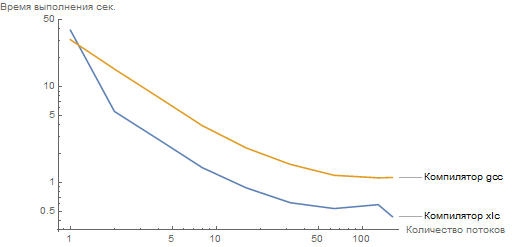
\includegraphics[width=0.7\textwidth]{plot_compilers.png}
\caption{Сравнение производительности программ собраных xlc и gcc}
\end{figure}
\par
В отличии от OpenMP программы на машине Polus разница между gcc и xlc незначительна и больше всего проявляется на максимальном числе процессов. Использование оптимизаций для xlc даёт ещё меньший, практически несущественный выигрыш. Для чистоты эксперимента были использованы исполняемы файлы полученные компиляторм xlc с максимальным уровнем оптимизаций.
\par
Для тестирования производительности были выполнены запуски по описанной выше методике с использованием двух конфигураций:
\begin{itemize}
\item Без оптимизаций
\item С предвычислением коэффициентов
\end{itemize}
\par
Были полученны следующие результаты:
\begin{table}[h]
\begin{tabular}{lllll}
Optimization & No          & Full       & No          & Full        \\
Series       & \multicolumn{2}{l}{1000} & \multicolumn{2}{l}{10000} \\
1            & 6.2305      & 2.76137    & 62.2856     & 27.6681     \\
2            & 3.14104     & 1.40206    & 31.3597     & 14.0333     \\
4            & 1.57998     & 0.705443   & 15.7431     & 7.06001     \\
8            & 0.794901    & 0.355019   & 7.87509     & 3.53876     \\
16           & 0.405254    & 0.179976   & 3.94487     & 1.77335     \\
32           & 0.0596141   & 0.0248764  & 0.508452    & 0.227737    \\
64           & 0.0360565   & 0.0152341  & 0.262685    & 0.117083    \\
128          & 0.0263095   & 0.0124611  & 0.13843     & 0.0621525   \\
256          &             &            & 0.0816035   & 0.0400828   \\
512          &             &            & 0.0614147   & 0.0374633  
\end{tabular}
\end{table}
\begin{table}[h]
\begin{tabular}{lllll}
Optimization & No           & Full        & No           & Full         \\
Series       & \multicolumn{2}{l}{100000} & \multicolumn{2}{l}{1000000} \\
8            &              & 35.3529     &              &              \\
16           & 39.3525      & 17.6991     &              &              \\
32           & 4.93753      & 2.22145     &              & 22.1799      \\
64           & 2.47605      & 1.11448     & 22.846       & 11.12        \\
128          & 1.24735      & 0.561337    & 11.6273      & 5.57871      \\
256          & 0.630394     & 0.283789    & 5.8362       & 2.79079      \\
512          & 0.332448     & 0.155836    & 3.523        & 1.39956     
\end{tabular}
\end{table}
\newpage
\par
Для наглядности на графиках:
\begin{figure}[h]
\centering
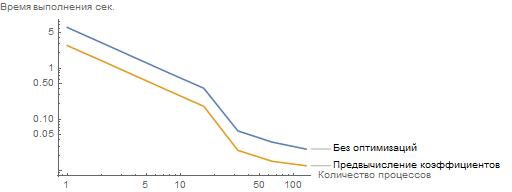
\includegraphics[width=0.7\textwidth]{plot1k.png}
\caption{Время выполнения для 1000 узлов}
\end{figure}
\begin{figure}[h]
\centering
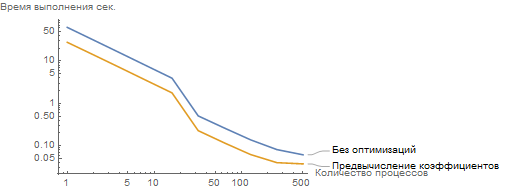
\includegraphics[width=0.7\textwidth]{plot10k.png}
\caption{Время выполнения для 10000 узлов}
\end{figure}
\begin{figure}[h]
\centering
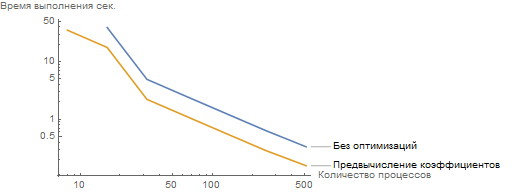
\includegraphics[width=0.7\textwidth]{plot100k.png}
\caption{Время выполнения для 100000 узлов}
\end{figure}
\begin{figure}[h]
\centering
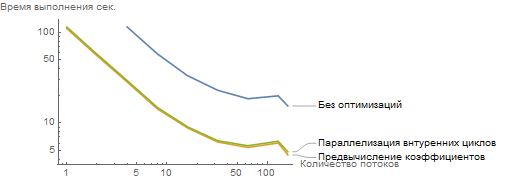
\includegraphics[width=0.7\textwidth]{plot1M.png}
\caption{Время выполнения для 1000000 узлов}
\end{figure}
\newpage
\section{Выводы}
Распараллеливание даёт значительный выигрыш как на большом так и на малом объеме данных. В отличии от OpenMP на комплексе Polus выигрыш в производительности есть на данных самого малого размера, и при увеличении числа потоков прирост производительности остаётся примерно тем же. Причиной этому могут служить как и большие накладные расходы на IPC в OpenMP, так и то что архитектура комплекса Blue Gene больше подходит для многочисленных MPI процессов, чем архитектура Polus для многочисленных OpenMP нитей. Также любопытно резкое снижение времени работы при переходе от 16 к 32 процессам, это может объясняться особенностью архитектуры узлов Blue Gene а также различными топологиями IPC. для разных объемов вычислений целесообразны разные параметры параллелизации. Так для 1000 и 10000 узлов имеет смысл использовать 64-128 процессов т.к. выигрыш от большего числа незначителен, в то время как для 100000 и 1000000 узлов имеет смысл задействовать доступные ресурсы по максимуму. 
\newpage
\section{Полный листинг программы} \label{source}
\subsection{Файл main.cpp}
\lstinputlisting[style = CStyle]{../main.cpp}
\subsection{Файл messaging.cpp}
\lstinputlisting[style = CStyle]{../messaging.cpp}
\subsection{Файл functions/arcsin.cpp}
\lstinputlisting[style = CStyle]{../functions/arcsin.cpp}
\subsection{Файл $functions/heaviside\_step.cpp$}
\lstinputlisting[style = CStyle]{../functions/heaviside_step.cpp}
\subsection{Файл functions/exp.cpp}
\lstinputlisting[style = CStyle]{../functions/exp.cpp}
\end{document}